%DO NOT MESS AROUND WITH THE CODE ON THIS PAGE UNLESS YOU %REALLY KNOW WHAT YOU ARE DOING
\chapter*{Experimental Research}
\addcontentsline{toc}{chapter}{Experimental Research}

\section*{ Rectangular Pulse } 
\addcontentsline{toc}{section}{Rectangular Pulse }
\noindent The spectrum of a rectangular pulse is shown in Figure 1. The output is obtained as a result of the Fast Fourier Transform algorithm using 512 points. Thus the frequency range corresponding to the time range on the left has been divided into 512 points in the spectrum on the right.The voltage of the spectrum is expressed in logarithm.

\noindent From the Figure 1, we can conclude that the Fourier transform of rectangular pulse is a sinc function in frequency domain. We know also from the Fourier transformation that the bandwidth of a rectangular pulse is given as $b = 1/T$ from this relation we deduce that $b*T = 1$ for all pulse durations. This CW signal exhibits some interference patterns in its ambiguity diagrams which could affect its range resolution. This pulse is having a good Doppler resolution which can be seen in the Figure 1.

\begin{figure}[H]
\centering
{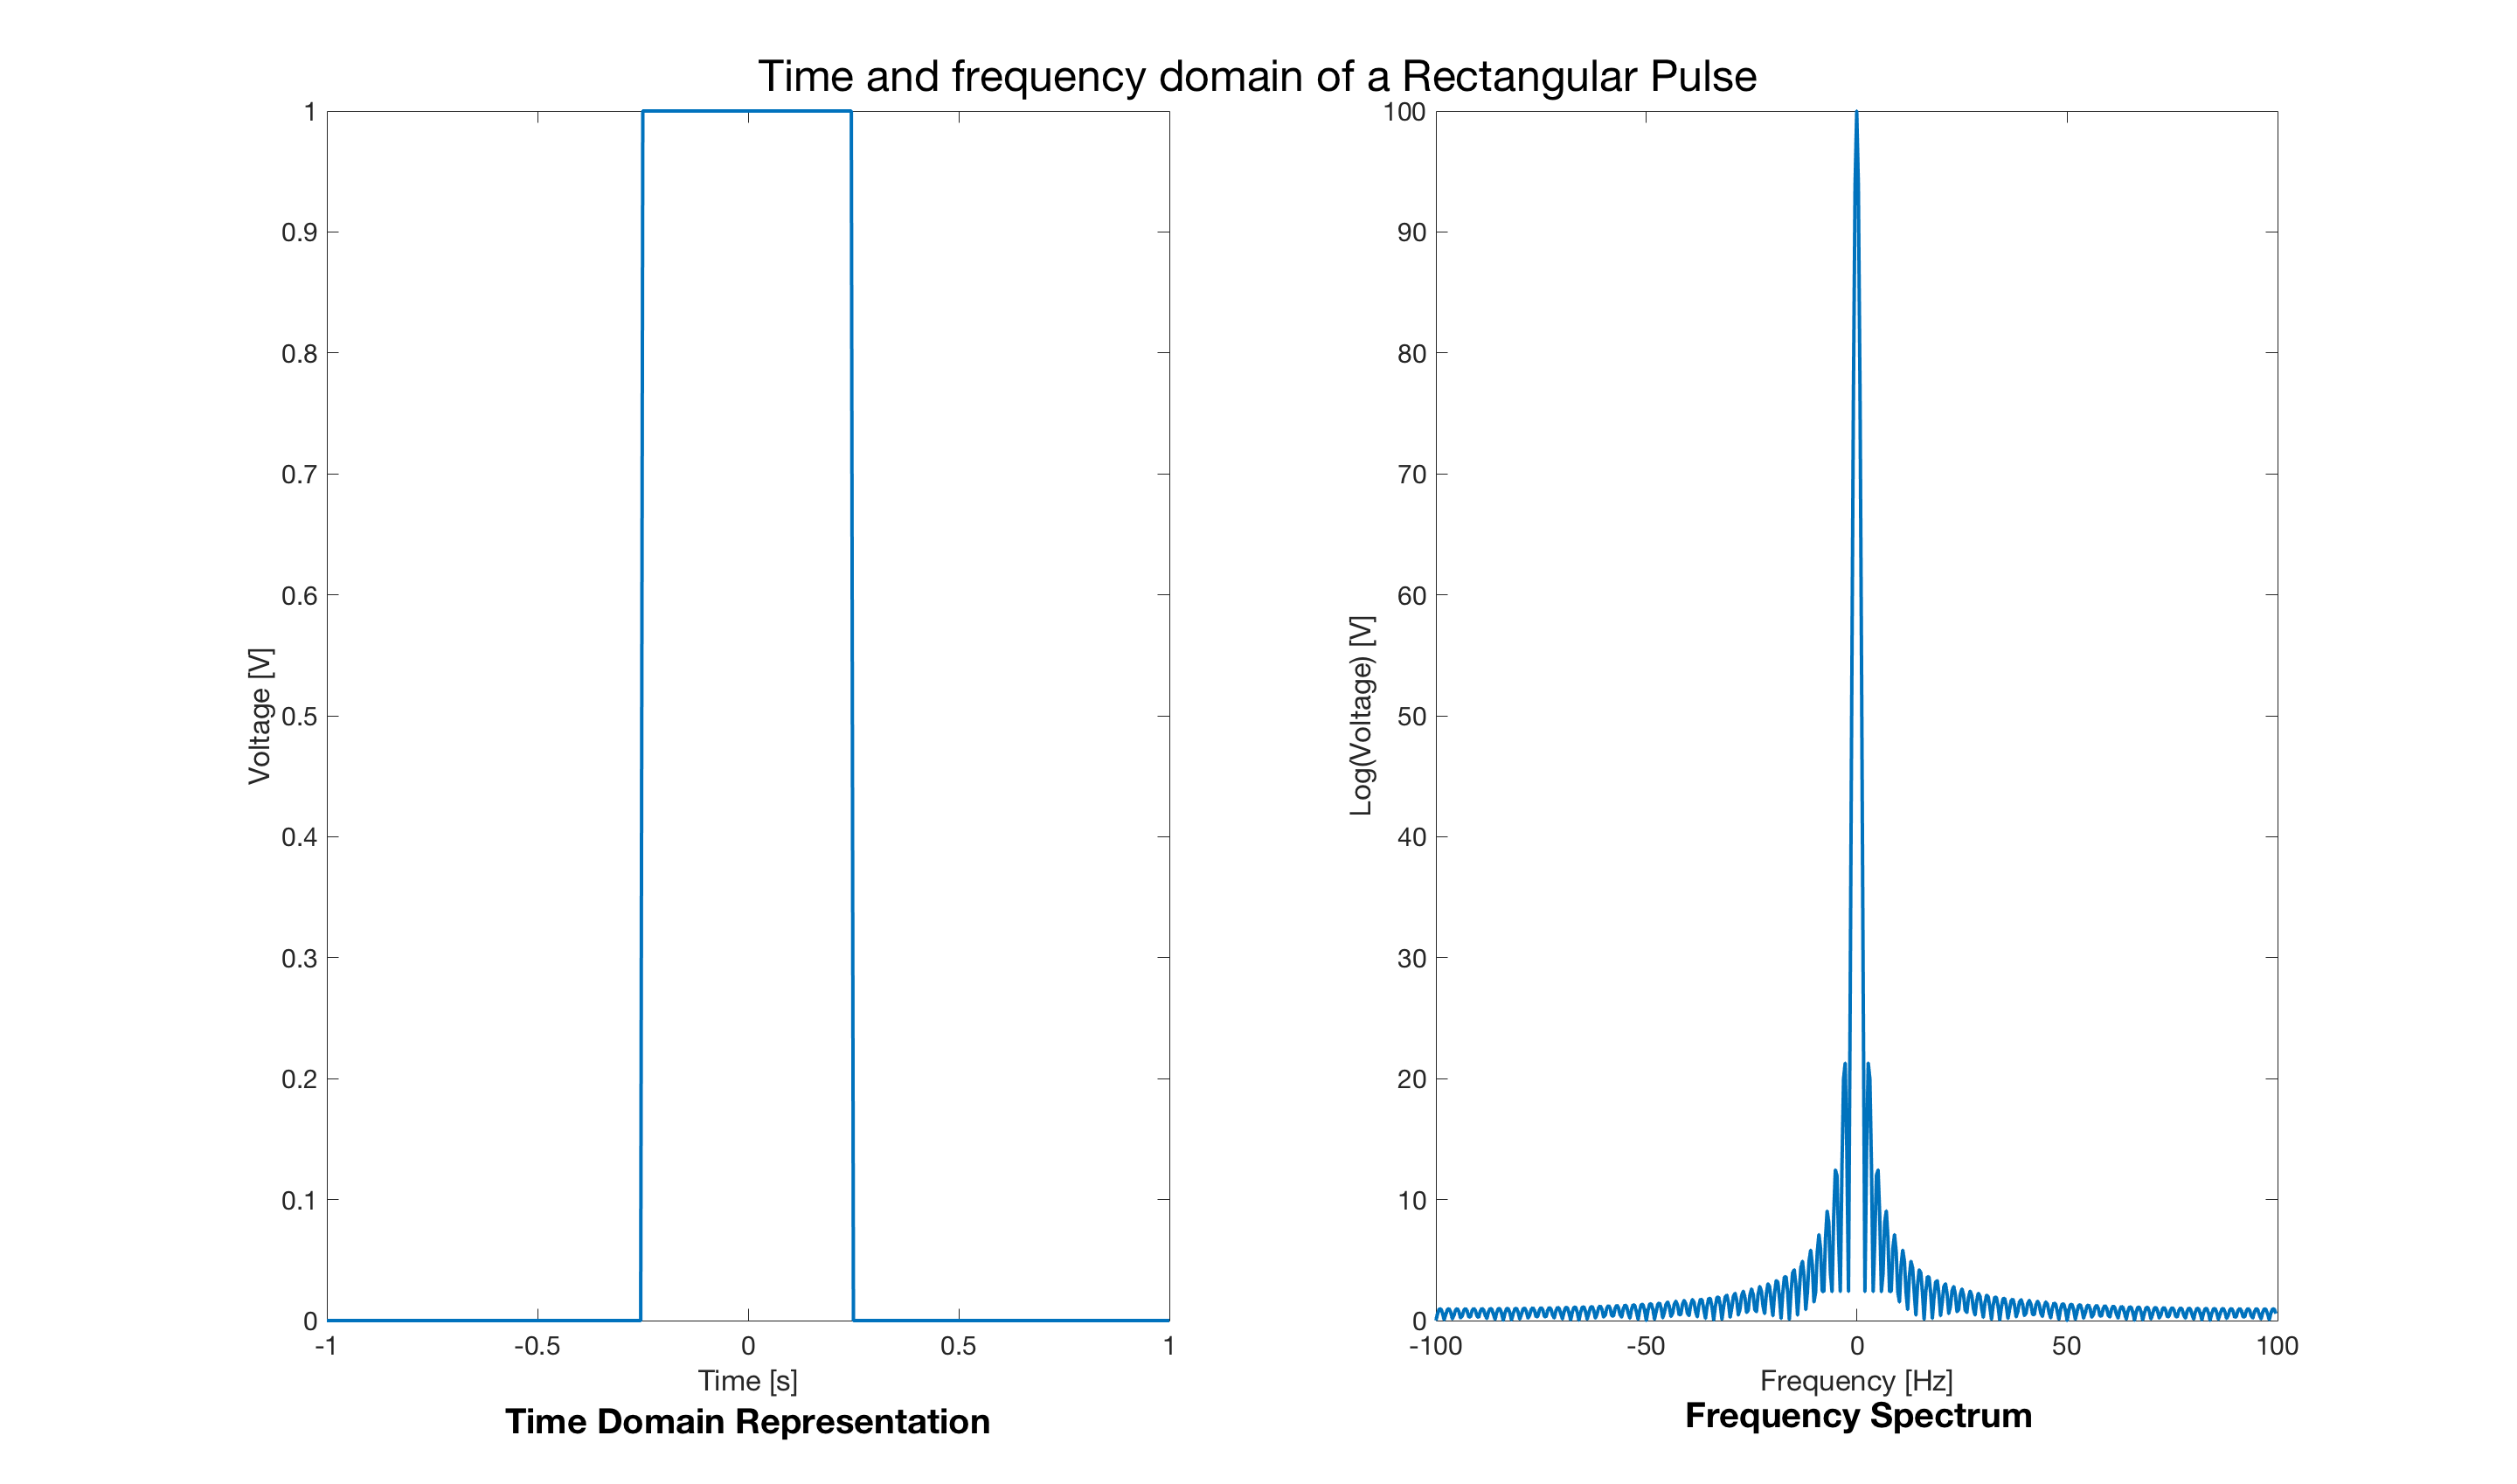
\includegraphics[scale=0.18]{usp8_1.png}}
\caption{ A rectangular pulse in time domain (left) along with its spectrum (right)}
\end{figure}

\noindent The ambiguity function plot above provides a three dimensional view of the amount of distortion that is involved with a rectangular pulse with a Doppler shift and a time delay. The peak value can be observed at the center while the values gradually decrease around the sides. This resembles a sinc function in three dimensions exactly like the Fourier transform of the rectangular pulse shown in Figure 1. In Figure 2 we can observe that the output of a matched filter depends on the Doppler Effect. We can also say that the range resolution of the rectangular pulse is relatively poor due to the zero Doppler shifts $(v = 0).$ T he matched filter produces a high output values for a big $\tau$ range. A lot of interferences could be observed for values of v$>$ 0.

\begin{figure}[H]
\centering
{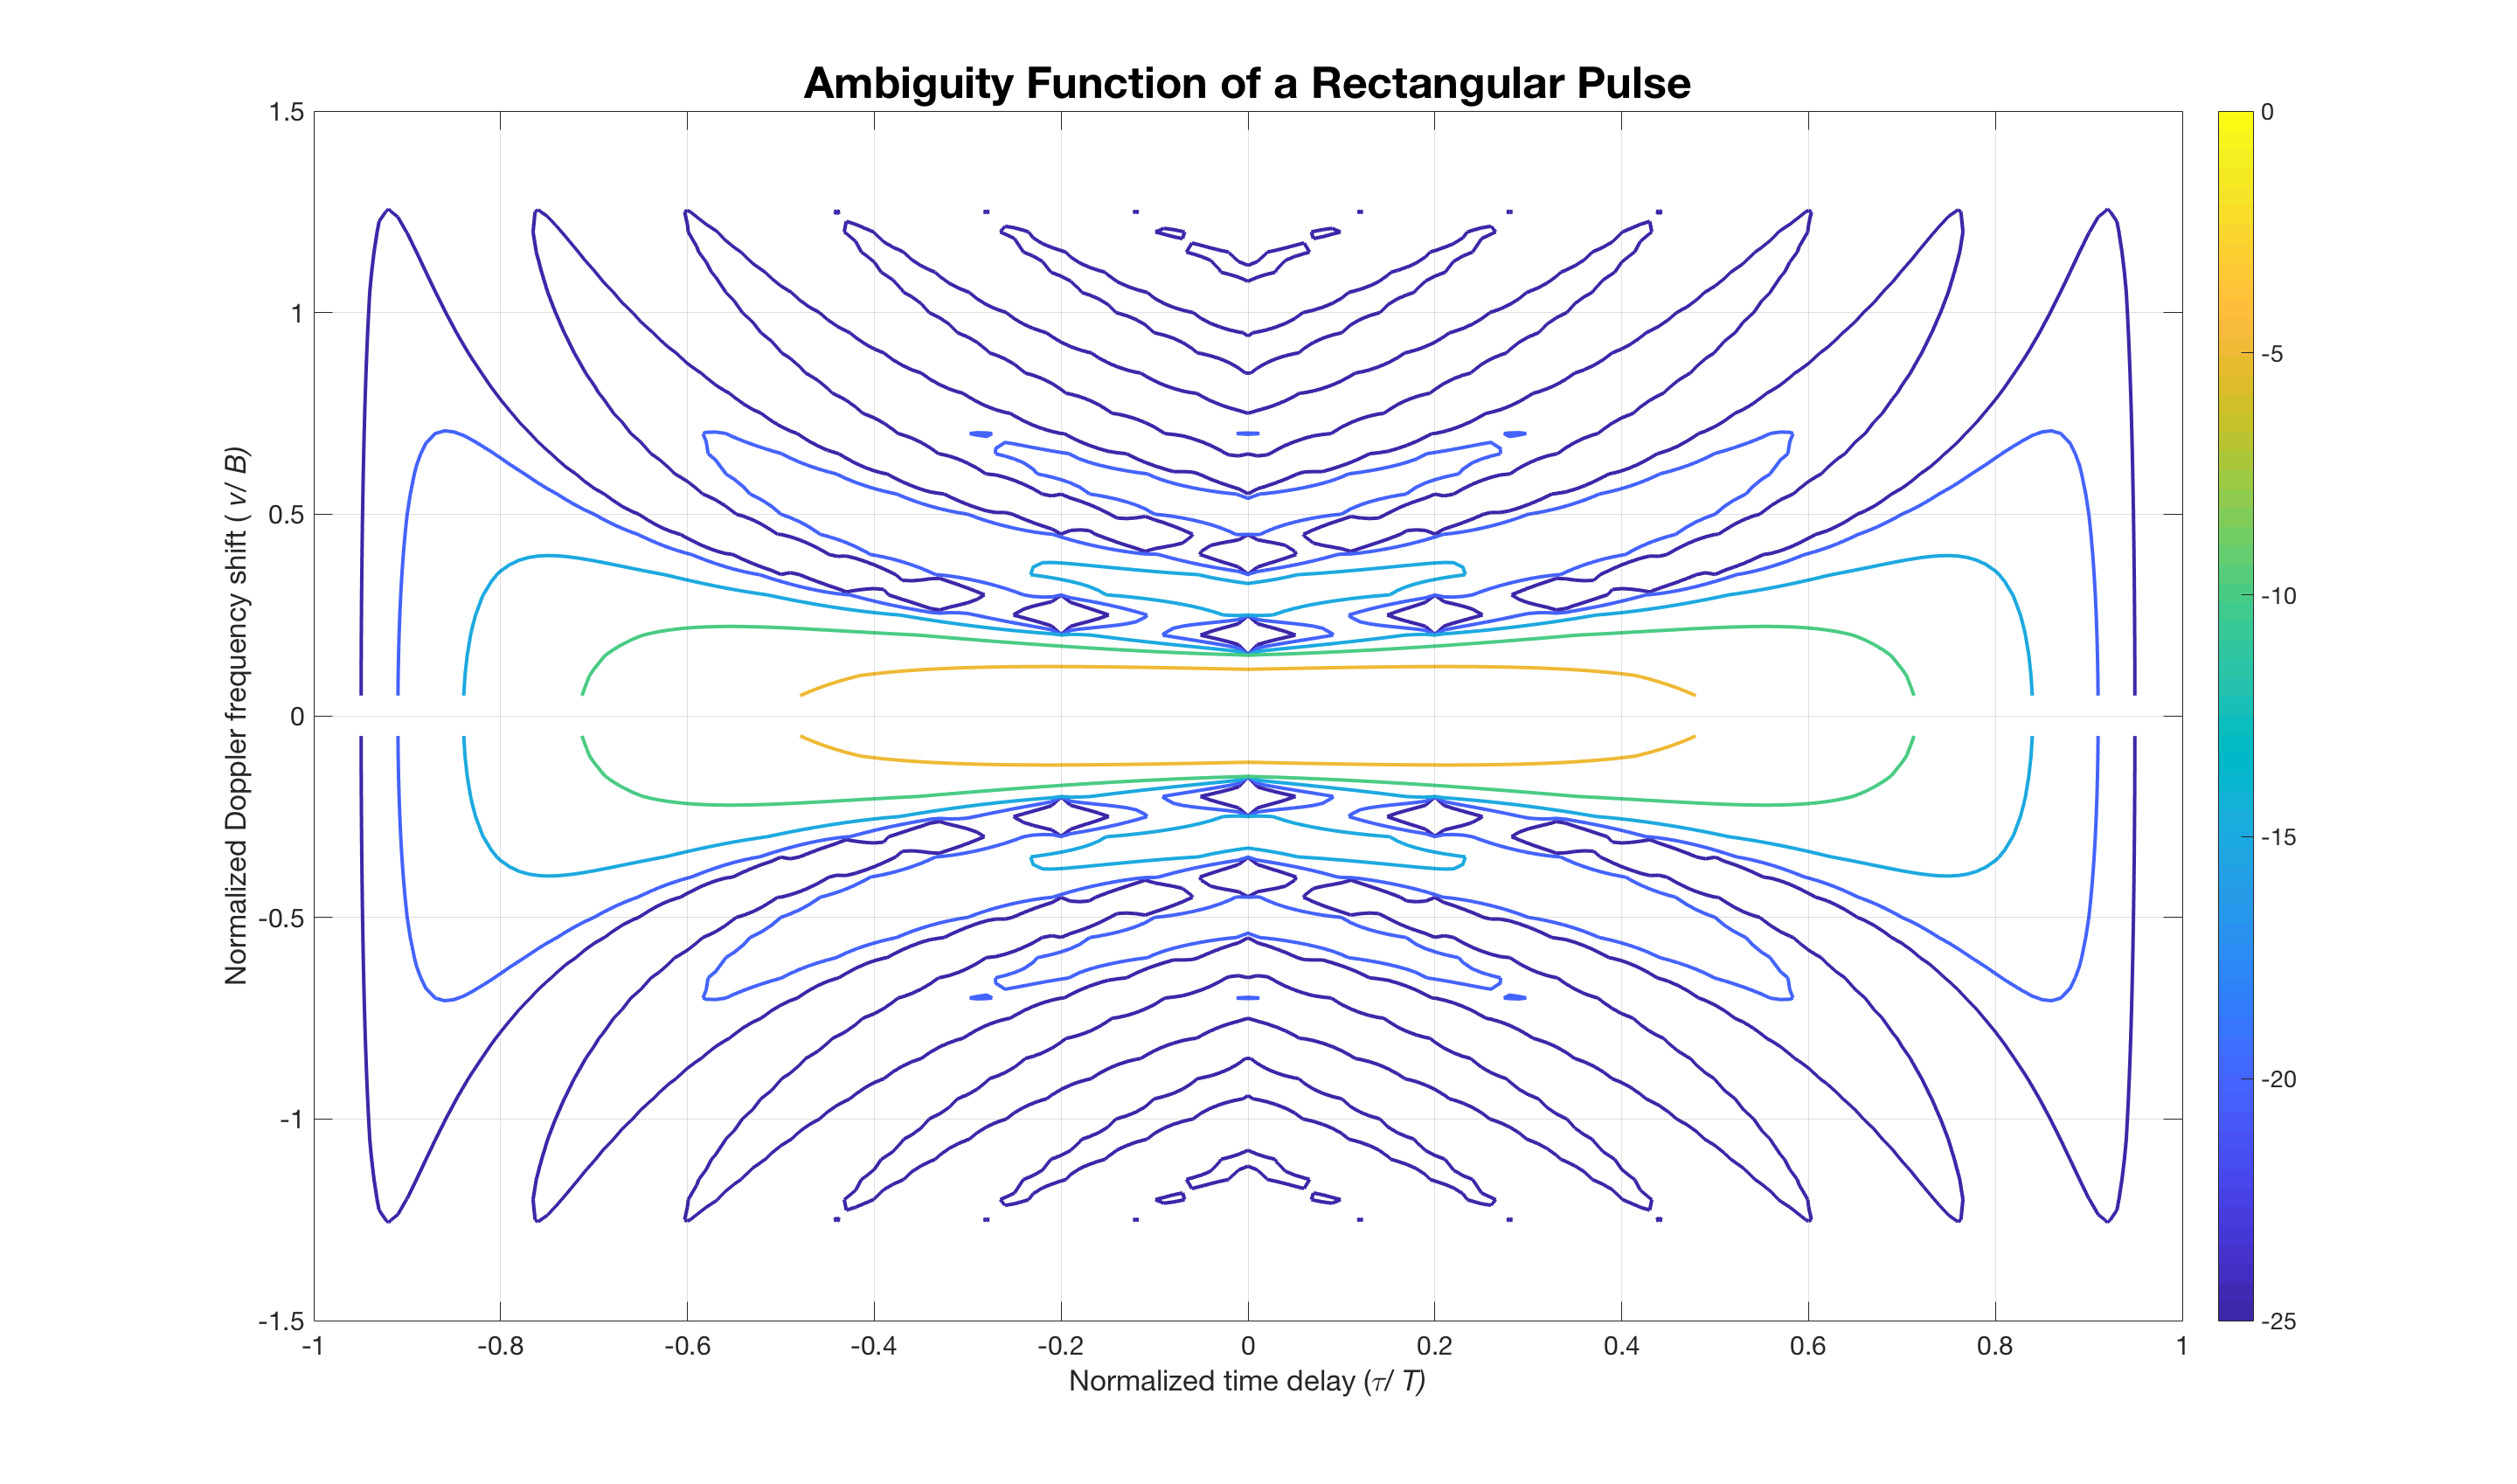
\includegraphics[scale=0.18]{usp8_4.png}}
\caption{ Ambiguity function of a rectangular pulse }
\end{figure}

\newpage
\section*{ Linear Frequency Modulated pulse with a Rectangular Envelope }
\addcontentsline{toc}{section}{Linear Frequency Modulated pulse with a Rectangular Envelope }

\noindent  Figure 3 displays the spectrum of a Linear Frequency Modulated pulse with a rectangular envelope. The voltage of the spectrum is expressed in logarithm.

\begin{figure}[H]
\centering
{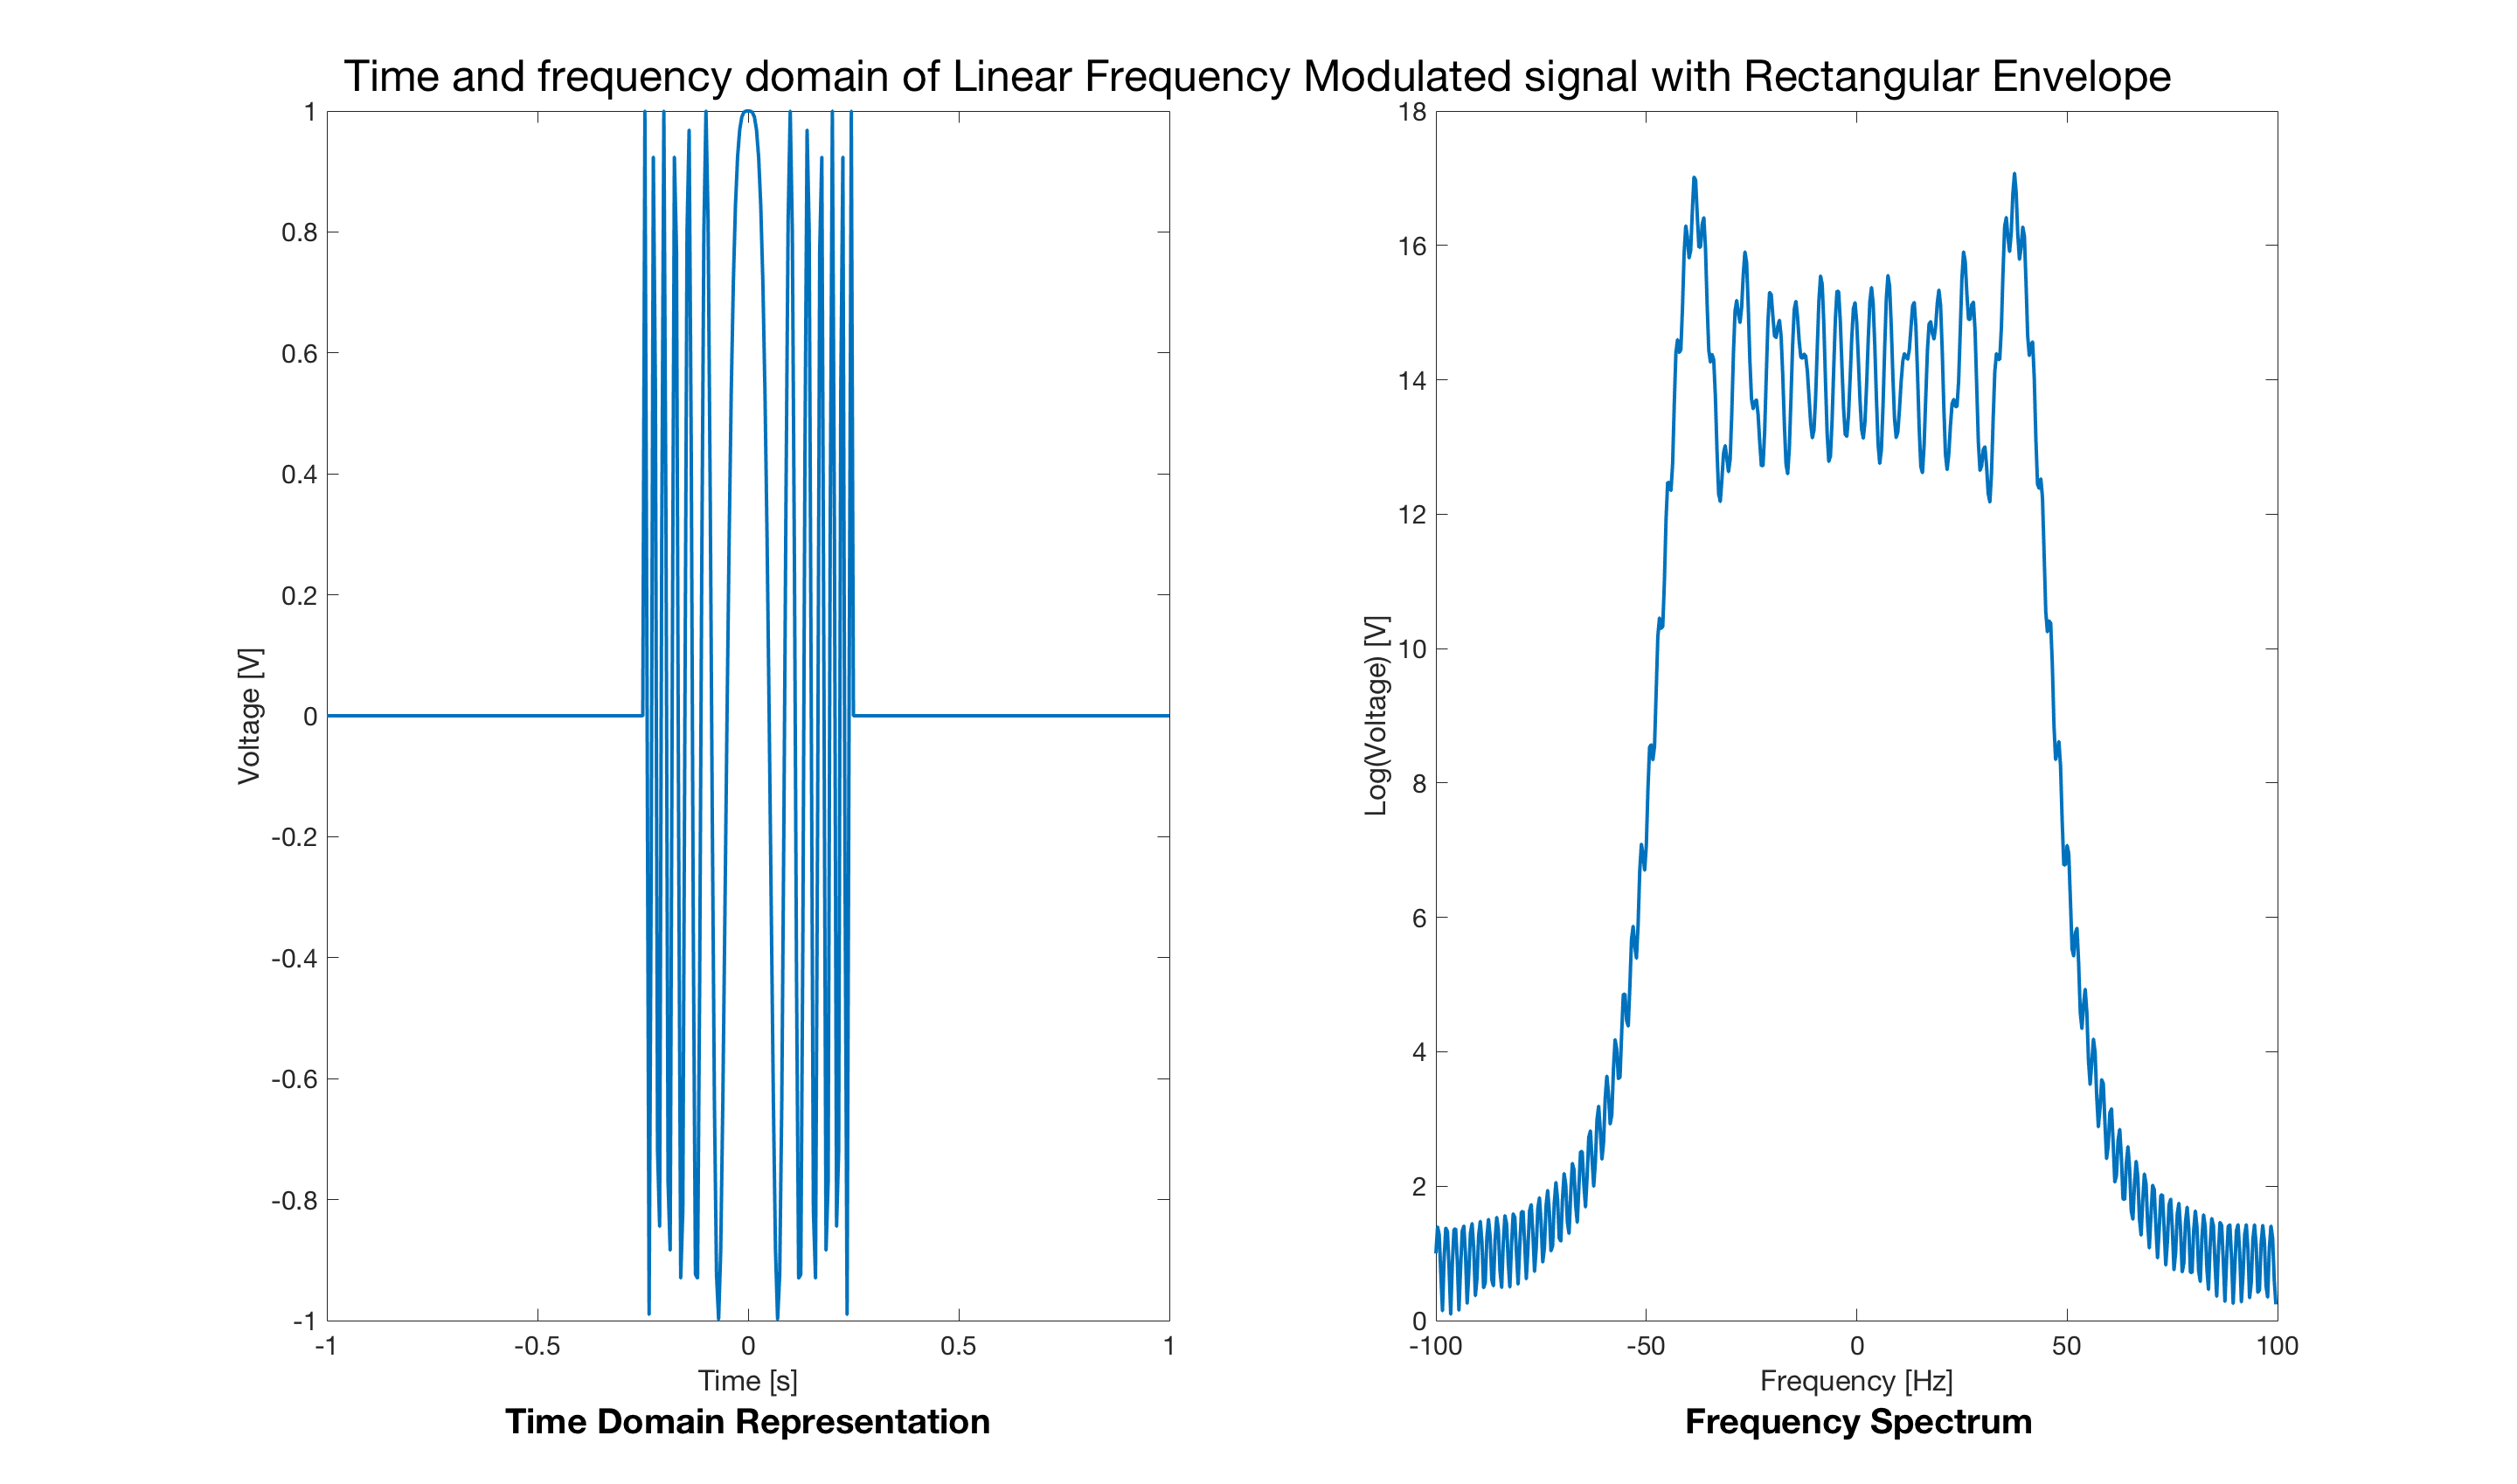
\includegraphics[scale=0.18]{usp8_2.png}}
\caption{ A Linear Frequency Modulated (LFM) pulse with rectangular envelope in time domain (left) along with its spectrum (right)}
\end{figure}

\noindent The signal shown on the left is a Linear Frequency Modulated pulse which is also known as a chirp. The Fourier Transform of a chirp with rectangular envelope is the figure shown on the right. The frequency variations can be seen in the peak of the spectrum around the center frequency.

\begin{figure}[H]
\centering
{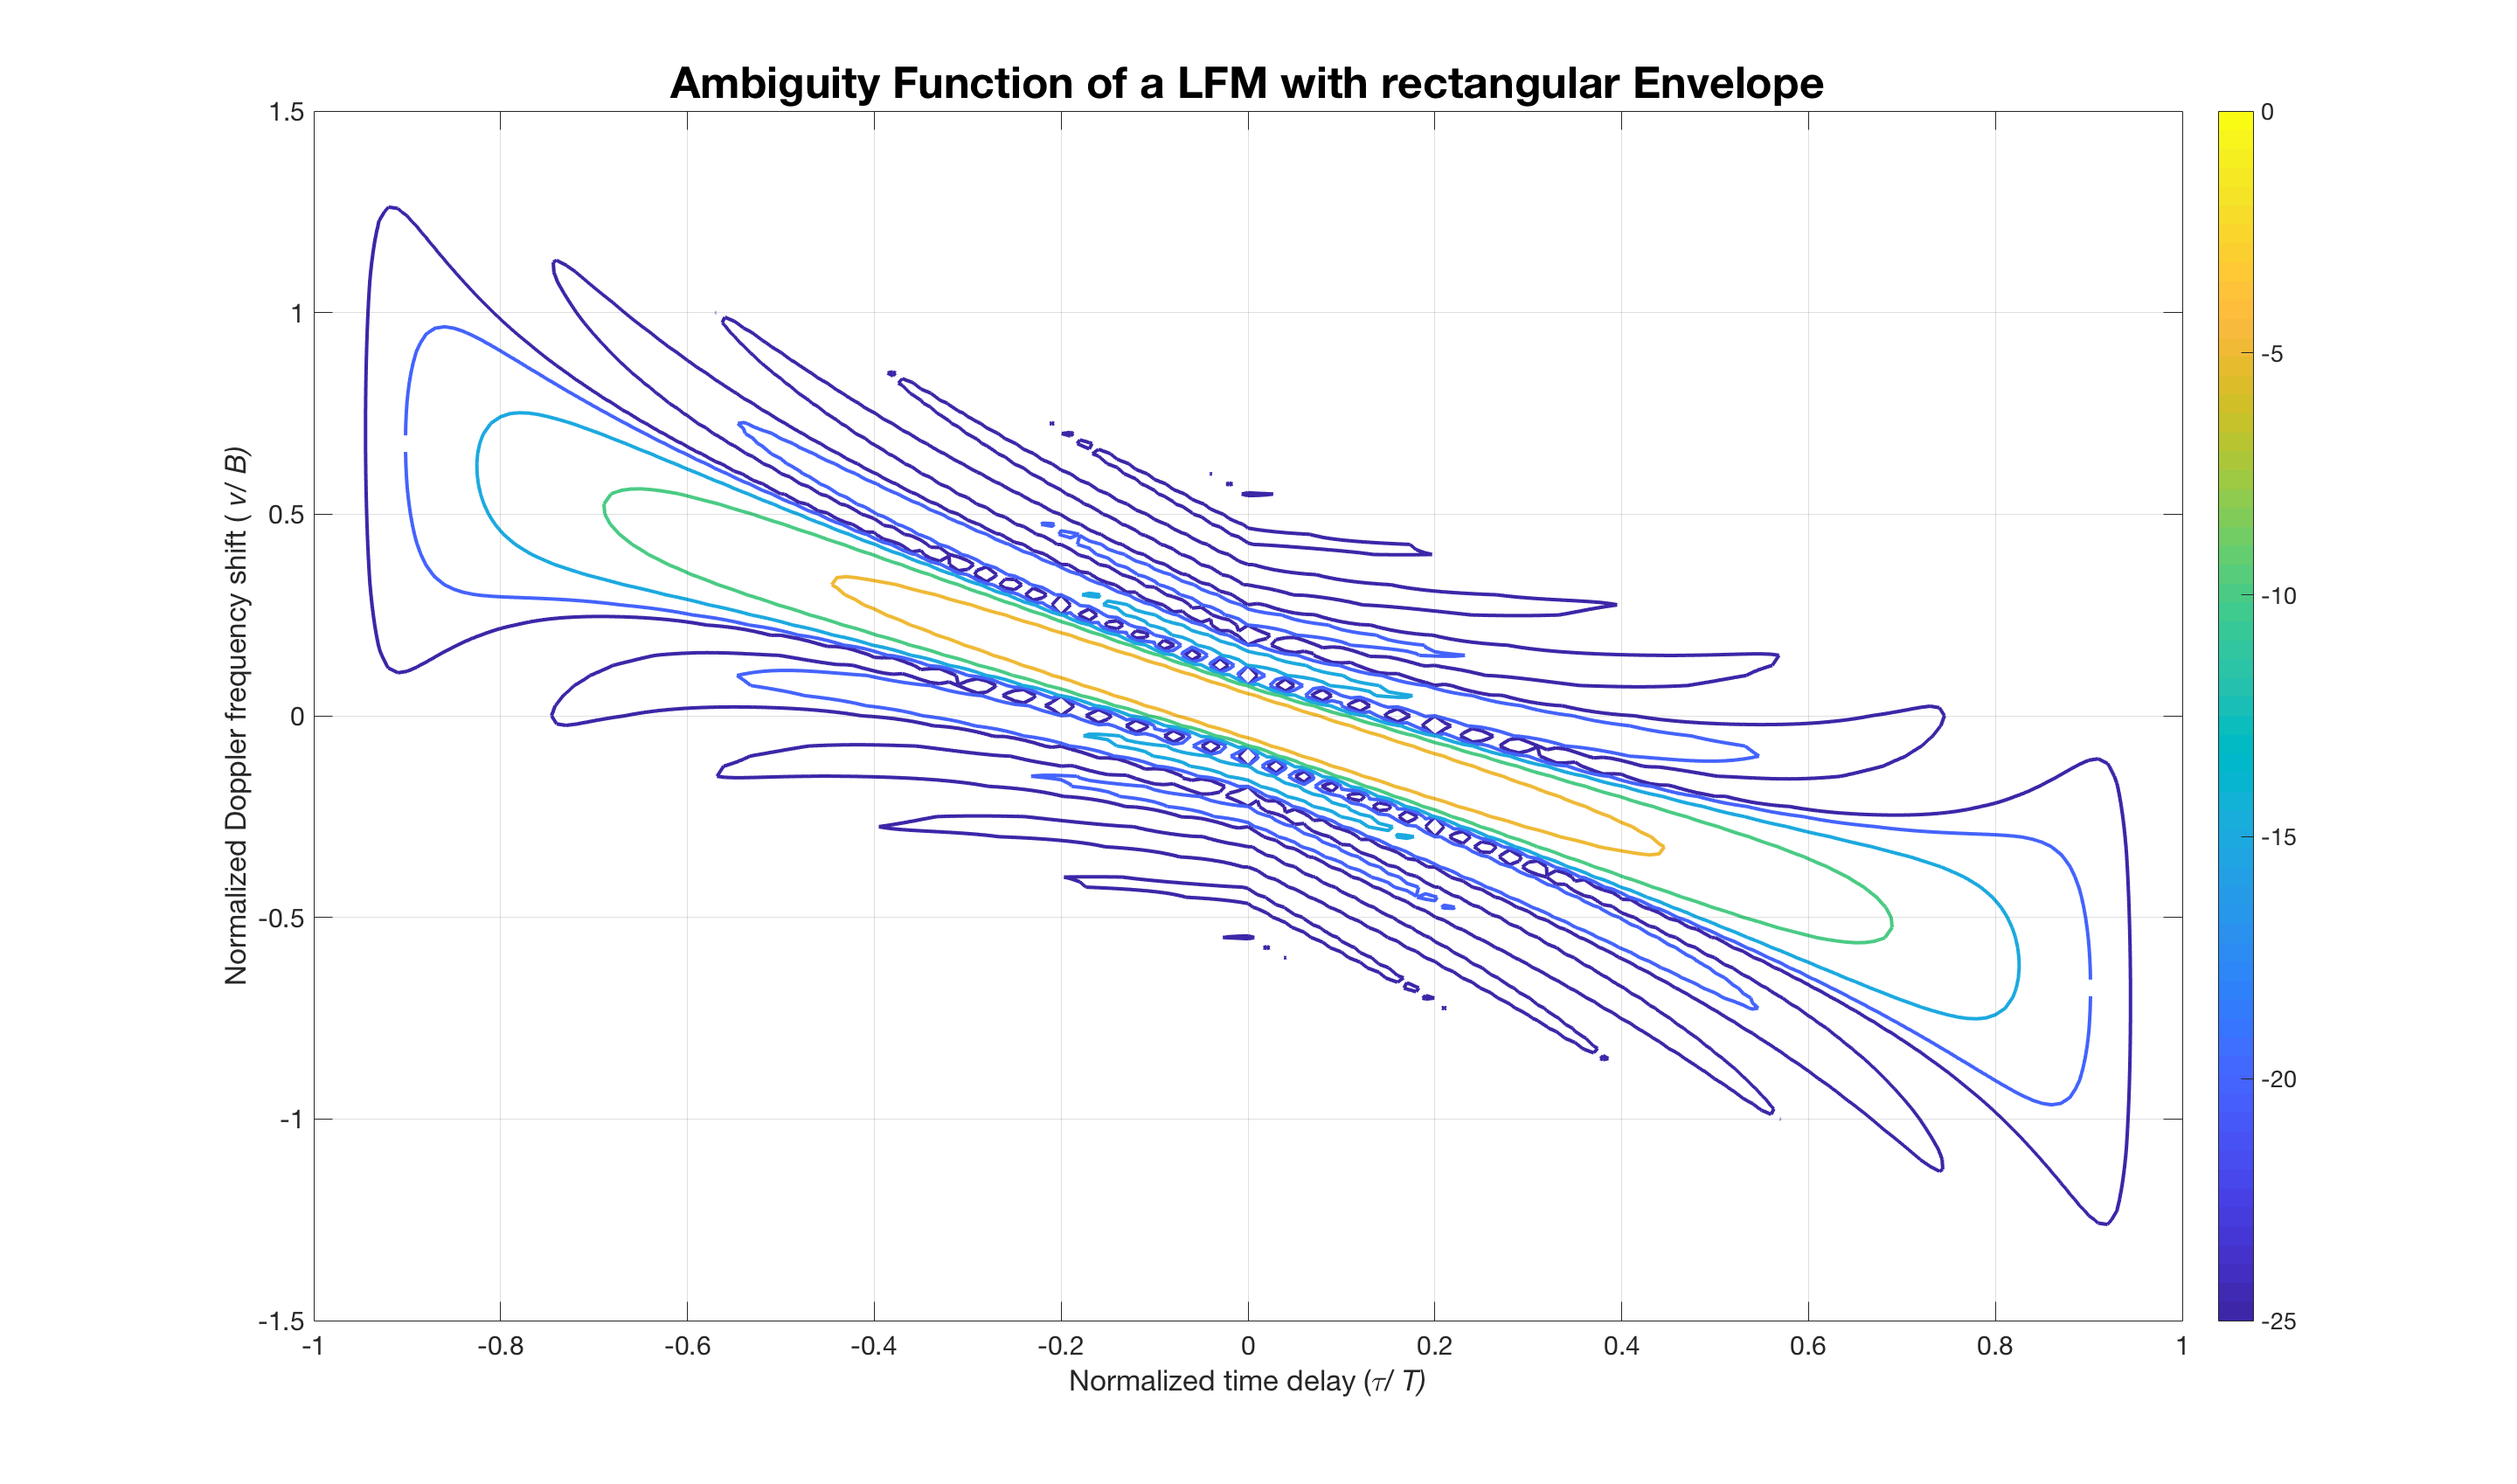
\includegraphics[scale=0.18]{usp8_5.png}}
\caption{ The ambiguity function of a Linear Frequency Modulated (LFM) pulse with rectangular envelope }
\end{figure}

\noindent  The spectrum and ambiguity functions in Figure 3 and Figure 4 are similar to that of Figure 1 when the slope of the FM signal is 0. So, the characteristics are also same. The slope of the FM signal (Figure 3) causes better range and Doppler resolution than the CW rectangular pulse (Figure 1).

\noindent The ambiguity function plot above shown above is similar to the one obtained for the rectangular pulse. The obvious change is the gradient observed in this figure which is due to the factor (k) introduced in the expression for the ambiguity function. The bandwidth time product for this pulse is $b * T = k * T^{2}$. The Figure 4 shows that the output of a matched filter has only a small dependency on the Doppler Effect. On the contrary, there are no problems with interferences in this case.
\newpage

\section*{Linear Frequency Modulated pulse with a Gaussian Envelope } 
\addcontentsline{toc}{section}{Linear Frequency Modulated pulse with a Gaussian Envelope }

\noindent Figure 5 displays the spectrum of a Linear Frequency Modulated pulse with a Gaussian envelope. The voltage of the spectrum is expressed in logarithm.

\begin{figure}[H]
\centering
{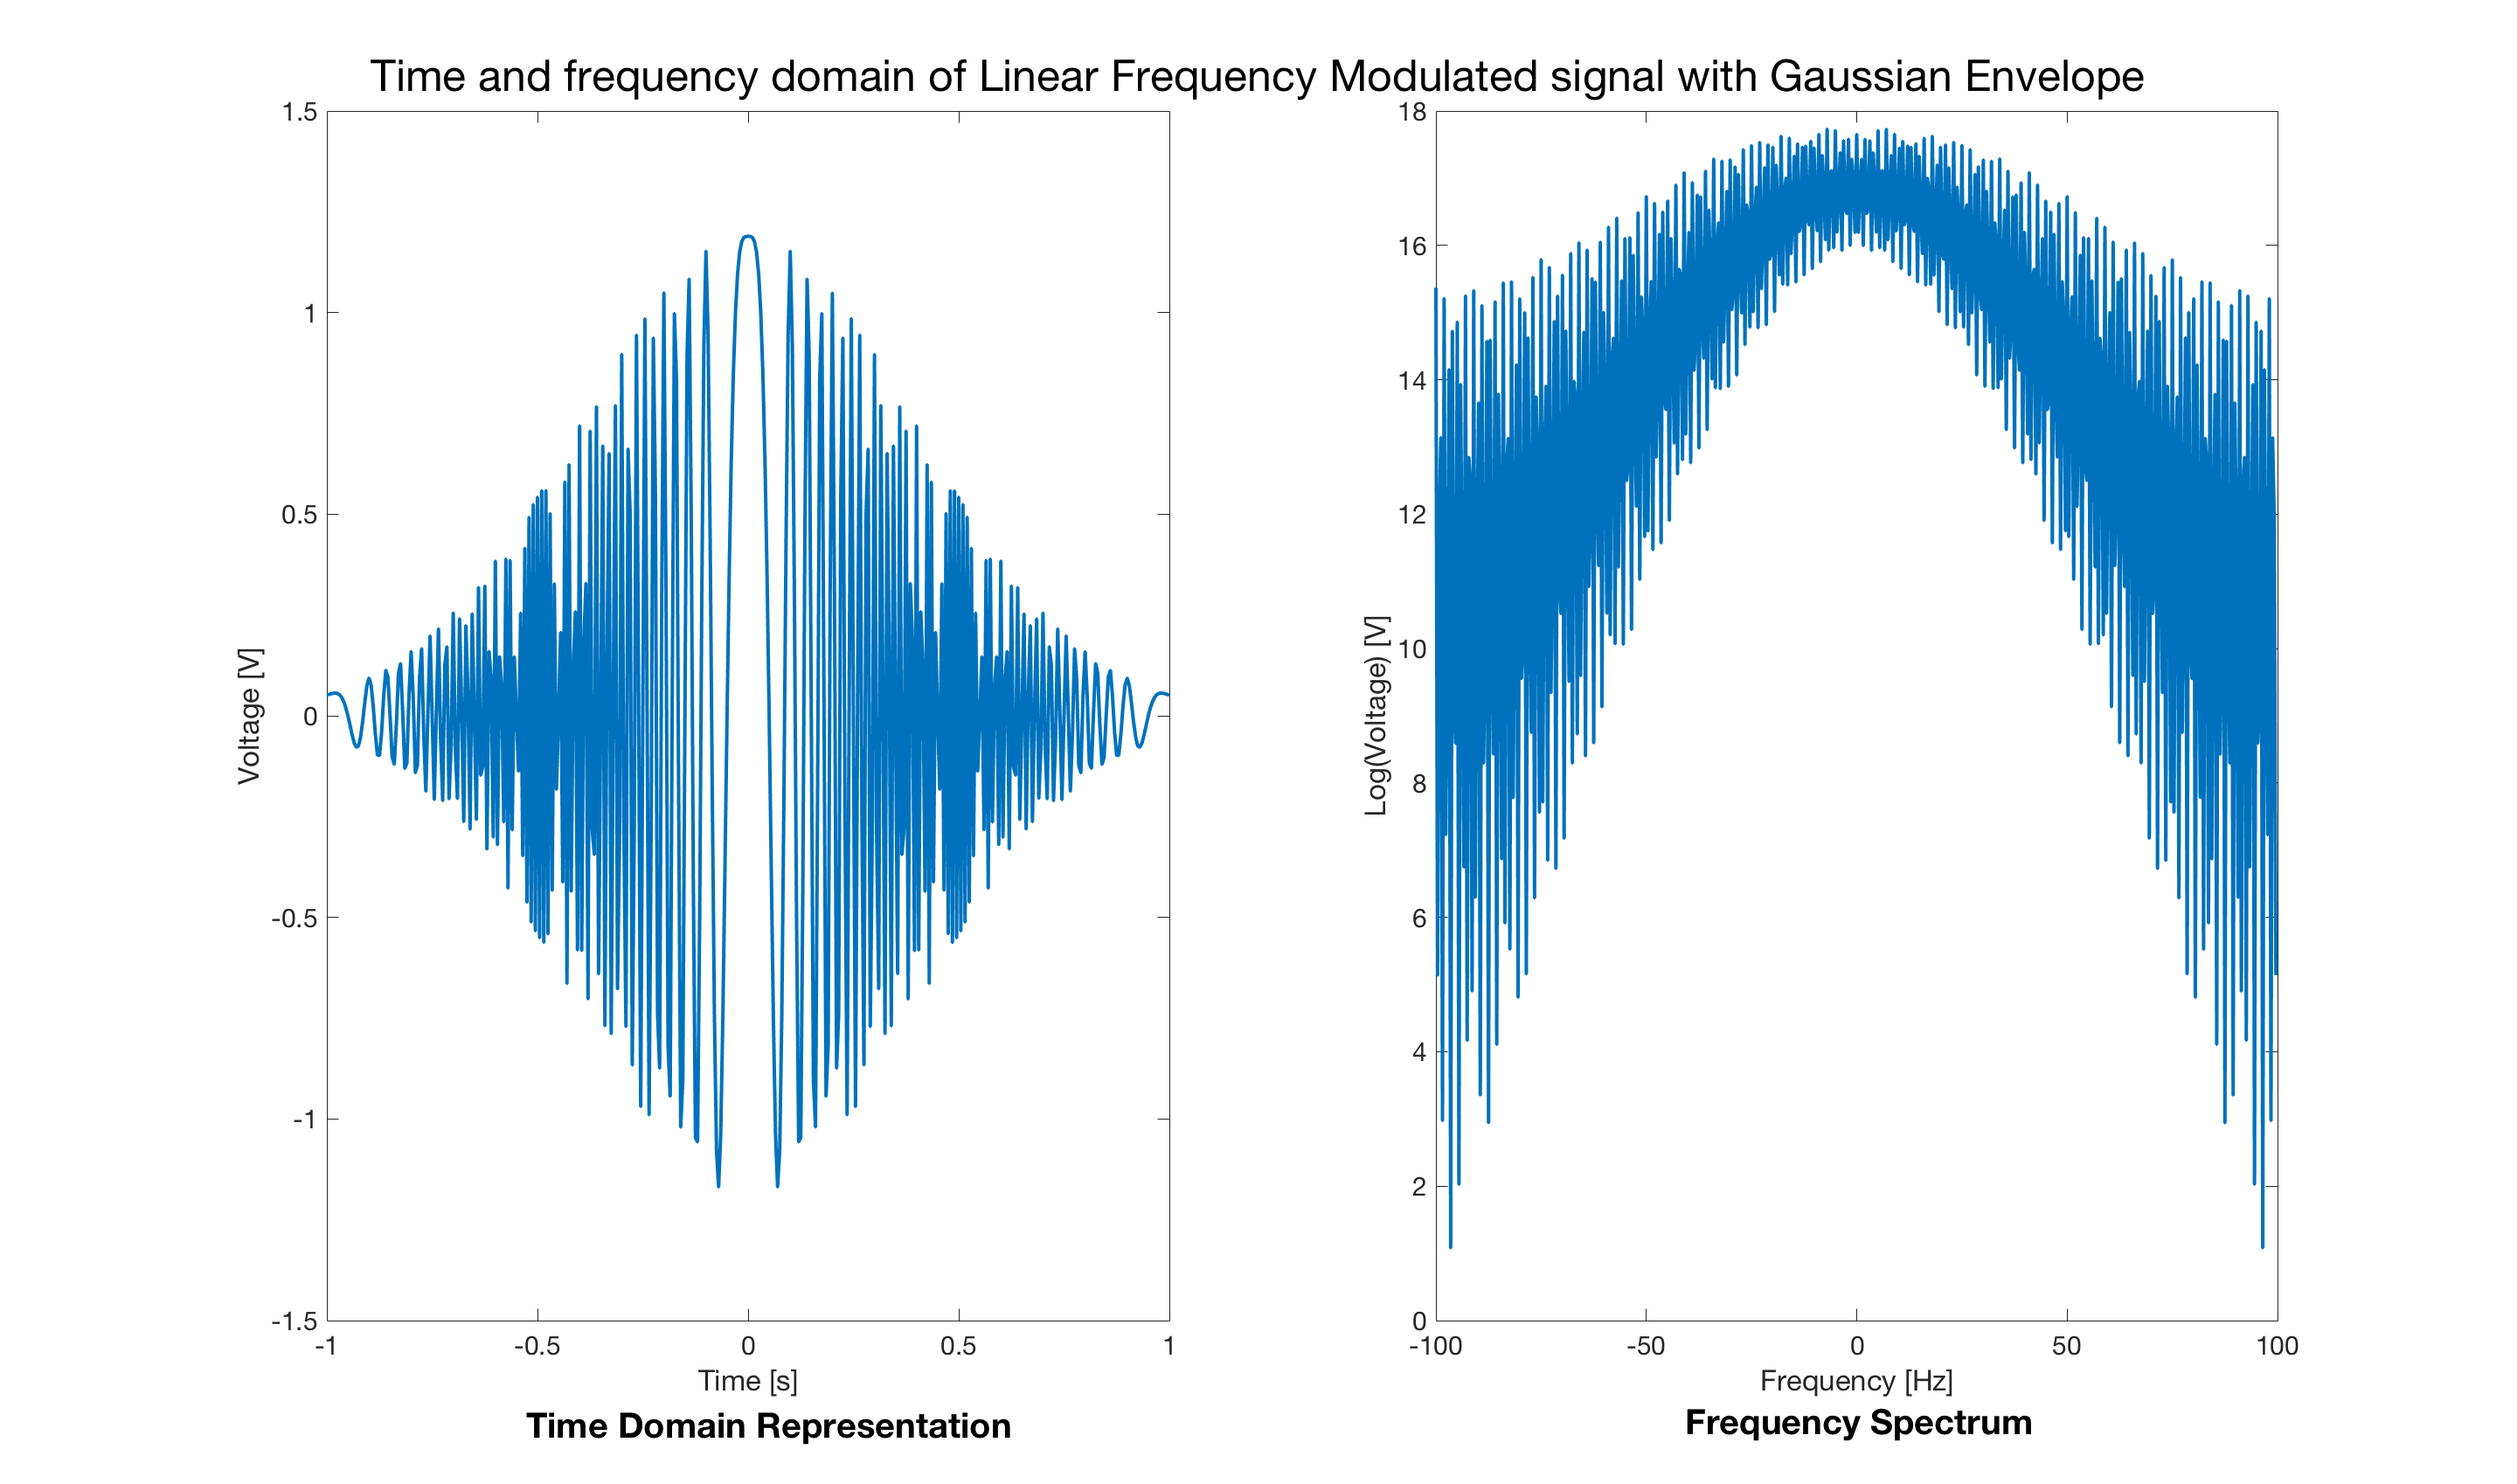
\includegraphics[scale=0.18]{usp8_3.png}}
\caption{ A Linear Frequency Modulated (LFM) pulse with Gaussian envelope in time domain (left) along with its spectrum (right)}
\end{figure}

\noindent The signal shown on the left is a Linear Frequency Modulated signal with a Gaussian envelope. The Fourier Transform of such a chirp is expected to yield a Gaussian envelope as is shown in the figure to the right. A Gaussian envelope with the frequency variations around it can be observed in the figure to the right.

\begin{figure}[H]
\centering
{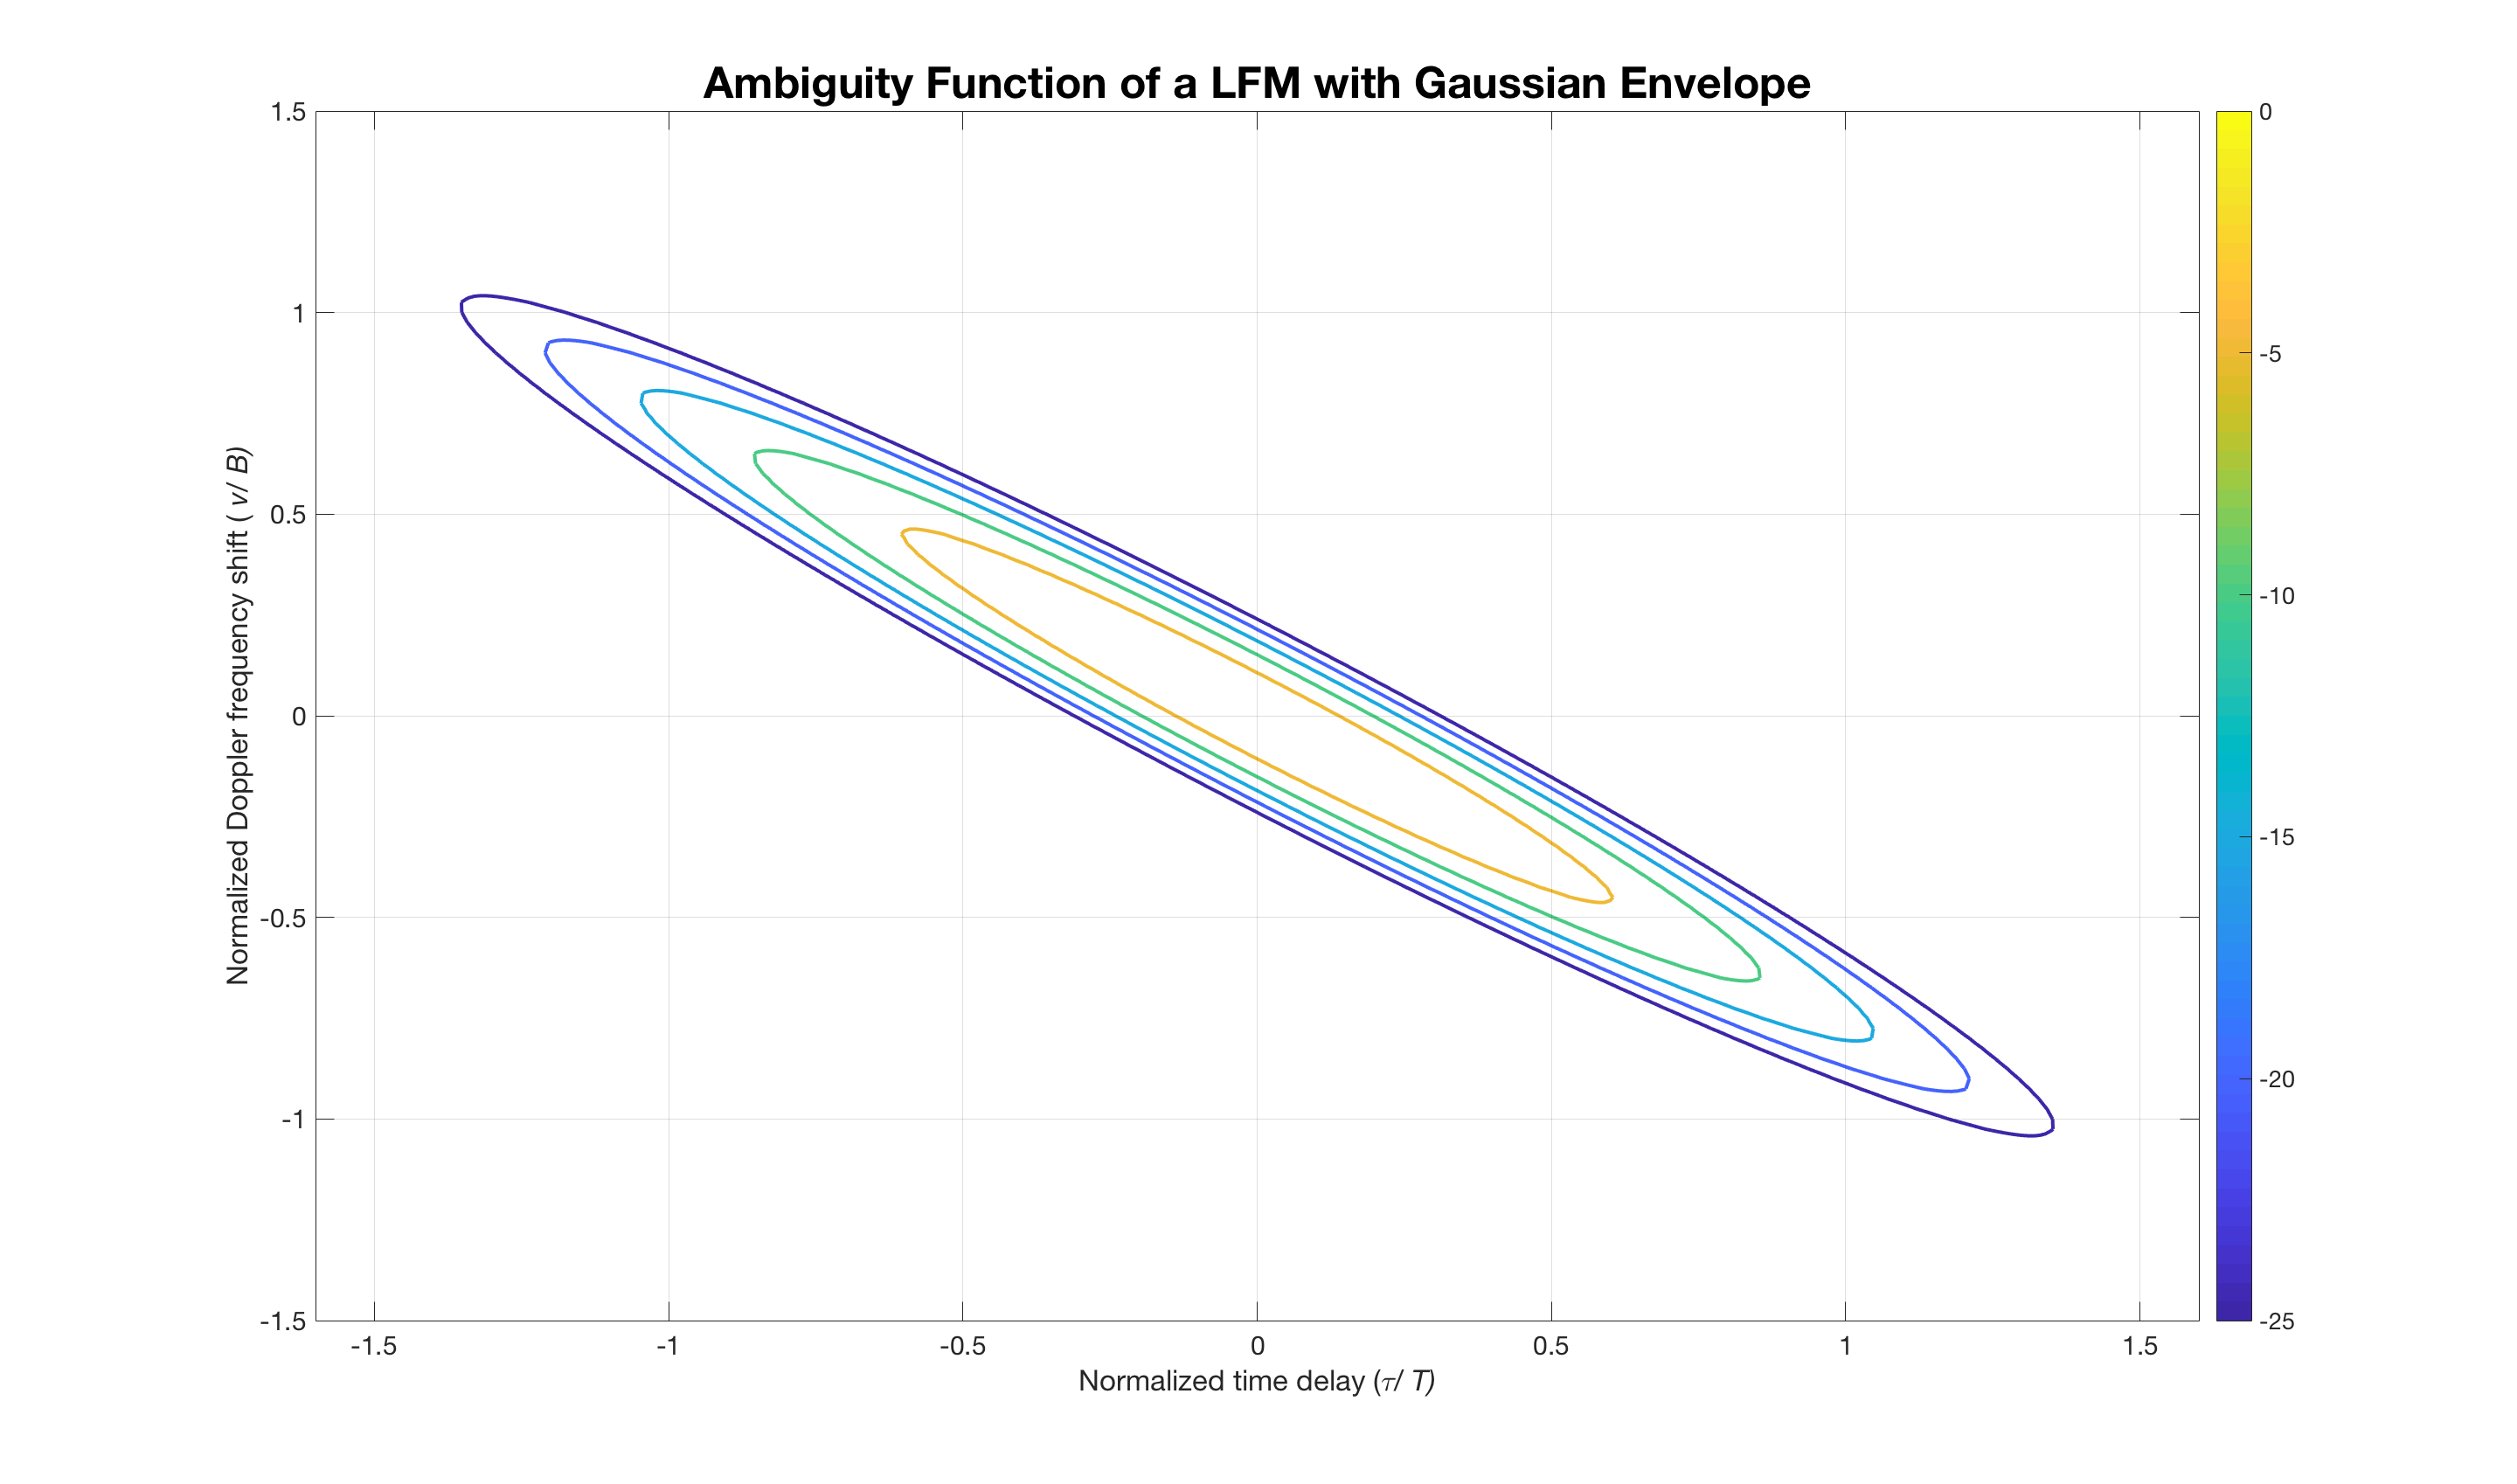
\includegraphics[scale=0.18]{usp8_6.png}}
\caption{ The ambiguity function of a Linear Frequency Modulated (LFM) pulse with Gaussian envelope }
\end{figure}

\noindent The ambiguity function plot shown above is similar to the spectrum of the LFM pulse with the Gaussian envelope. The three dimensional representation shown above also has a Gaussian shape with the peak around the center frequency.

\noindent Interference is not present as compared to the rectangular pulse. Furthermore, slope of the FM signal increases the range and Doppler resolutions considerably. The bandwidth time product for this pulse is $2 b*T = k *T.$ In Figure 6, we can observe that the output of a matched filter has only a small dependency on the Doppler Effect. 
